%%% EXPERIMENTAL HEADERS
% \usepackage{fancyhdr}
\pagestyle{fancy}
% \fancyhf{} % clear all header and footer fields
\fancyhead[CE]{R~A~T~I~O~N~A~L~~~~T~H~A~U~M~A~T~U~R~G~Y} 
\fancyhead[CO]{CHAPTER \thechapter: \leftmark}
% \fancyfoot[LE,RO]{\thepage}
\renewcommand{\chaptermark}[1]{\markboth{\MakeUppercase{#1}}{}}
\renewcommand{\headrulewidth}{0.4pt}
% \renewcommand{\footrulewidth}{0.4pt}
%%%%
\begin{savequote}[75mm]
It is the organization of a piece which helps the listener to keep the idea in mind, to follow its development, its growth, its elaboration, its fate.
\qauthor{Arnold Schönberg\footnote{\citet[381]{schonberg}}}
\end{savequote}

\chapter{Introduction}
\pagenumbering{arabic}
\label{introduction}

% \lettrine[lines=2,slope=-2pt,nindent=2pt]{\textcolor{SchoolColor}{O}}{n March 11, 2020}

\lettrine[lines=3]{\setmainfont{GoudyInitialen}[Path=./fonts/, Extension = .ttf]\color{printGreen}O}{n March 11, 2020} my first string quartet Hamonshū\index{Evans, Gregory Rowland!compositions!\textit{Hamonshū}} was premiered by the JACK quartet\index{JACK Quartet} alongside the works of several of my classmates in the composition department at the University of Iowa. While I was incredibly proud of the entire concert, I felt a slight uneasiness at the similarity between all of the works. When requesting feedback from some of my mentors and colleagues, one criticism stood out: the criticism that the piece did not have a clear formal arc. The work consists of seven relatively static panels of texture. As I listened back to each of the pieces on the concert, I found that this was what I had perceived as the connecting thread of similarity. The works were not activating my sense of memory through their formal architecture.\marginpar{Nevertheless, I was deeply inspired by the beauty of these works and I have been lucky to be able to interact with such talented colleagues.}

%\marginpar{The formatting of the margin paragraph definitely leaves something to be desired. It is good for informal, brief asides.}

\section{Origins}

In the course of my composition studies during both of my previous degrees, I summarized my growth in one primary technique. As an Undergraduate I spent most of my time learning how to create interesting musical materials, not just through harmonic and rhythmic innovation, but also by having a deep connection to the physical properties of the instrumental apparatus and even electronic manipulation of sound. As a Master's student, I developed a strong framework for compositional formalization in the Python\footnote{\url{https://www.python.org/}} programming language through the use of the Abjad\footnote{\url{https://abjad.github.io/}} \ac{API} for \ac{FSC}. This allowed me to develop rigorous systems for material generation which could be directly exported as Lilypond\footnote{\url{https://lilypond.org/}} files, cutting down the timeline required to compose formalized music.\marginpar{Obviously I learned more than one thing from each of my mentors.} After the premiere of Hamonshū\index{Evans, Gregory Rowland!compositions!\textit{Hamonshū}} I decided that the main field of compositional inquiry I needed to pursue during my Doctoral studies would be understanding the nature of the dramatic arc of large-scale formal systems. I was specifically searching for a way to approach the manipulation of aspects of form which could be integrated into my understanding of musical modernism.

I have never felt that I have understood the expressive role of the composer in modernity and as a result, I have been looking for systems which allow me to feel like I am in control of my music. Certainly, aspects of creative practice are perplexing or mysterious, even to the artist, but I found myself genuinely dumbfounded as to what I was doing when I sat down at my desk to compose. Gradually, I developed perspectives on rhythm, harmony, orchestration, and performing techniques, all within a highly rational framework. However, the question of how to deal with large-scale formal changes eluded me. In fact, I was resistant to the idea of allowing any ``changes'' in the flow of my music at all. This would mean that some elements of the work would not be developmentally related to one another. I eventually abandoned this need for total material inter-connectivity due to my experience with the music of two specific composers. In this dissertation, after a brief discussion of a negative example: Jean Barraqué's \textit{Sonate pour piano},\index{Barraqué, Jean!compositions!\textit{Sonate pour piano}} I will analyze two works which have had a significant impact on the way I think of composing large-scale forms: \textit{Rhea} by Francsico Guerrero\index{Guerrero Marín, Francisco!compositions!\textit{Rhea}} and \textit{Akasha}\index{Baca, Trevor!compositions!\textit{Akasha}} by Trevor Bača. In the works, the rational ordering of events of distinct genetic origin provide a formalist approach to large-scale form rather than the static uniformity of much early modernist music. These works suggest to me that the use of multiple generative processes within a work is not contradictory to the project of formalization. These pieces first interested me because I felt I could hear their structures. They gave me a psychological sensation of \textit{feeling} the form come into being in both the \textit{pro}gnostic and \textit{retro}gnostic fields of my memory while still engaging with the language of musical modernism. After the analytic chapters, I will summarize the shared characteristics of two of my own works, \textit{Polillas}\index{Evans, Gregory Rowland!compositions!\textit{Polillas}} for string quartet and \textit{Alu} for sinfonietta.\index{Evans, Gregory Rowland!compositions!\textit{Alu}}

\section{Modernism}

I decided to study form in contemporary music because of certain compositional trends which I noticed in contemporary music associated with the avant-garde. The Schönbergian approach to atonal pitch construction, specifically the twelve-tone system, is deliberately oriented toward a disintegration of tonal hierarchy,\footnote{\citet[207]{schonberg}} replacing tonal syntax with a new structuring principle which can often produce a sense of undifferentiated, saturated harmonic space.\footnote{\citet[39]{stockhausen}} This challenges the composer to organize musical discourse in ways other than through tonal pitch-centricity. When learning to analyze form in tonal music, it is the cadence which most clearly signifies the boundaries between themes,\footnote{\citet[34]{white}} but without cadences these sections could be better identified by their motivic content — in William Drabkin's article ``Theme'' in Grove Music Online, he makes the comment that the 12-tone series of a composition could \textit{itself} be considered the theme of a work and all statements of the series are developments or variations of that theme.\footnote{\citet{grove}} Likewise, the audience is also forced to listen for different orienting qualities.\index{Baca, Trevor}
\index{Barraqué, Jean}
\index{Boulez, Pierre}
\index{Evans, Gregory Rowland}
\index{Ferneyhough, Brian}
\index{Guerrero Marín, Francisco}

In the era of pointillistic music, reaching its culmination during the 1950's, the same kinds of approaches used to liberate harmony from cultural referentiality were applied to other sonic dimensions, for instance serializing rhythmic durations to disintegrate expressionist gestural vocables.\footnote{\citet[22]{ferneyhough}} After the surge of point-music, several modernist composers seemed to be looking for alternatives to compositional methods which proliferate musical ideas from a single motivic kernel.\footnote{\citet[81]{griffiths}} Stockhausen developed his theory of groups, Xenakis developed statistical composition, and some composers developed, after Stravinsky, what Jonathan Cross calls \textit{block forms}.\footnote{\citet[20]{cross}} These developments encouraged me that modernist thinking does not, by necessity, produce music with the æsthetic of sameness, rather contrast and differentiation can be controlled with the same level of precision as other facets of the musical surface.

\subsection{Is there a good definition of modernism?}

It is difficult to precisely define musical modernism\footnote{\citet[15]{legacy}} or even modernism as a whole.\footnote{\citet[2]{oxford-modernisms}} Recent developments in the study of modernism reveal a picture of an artistic movement of many, sometimes contradictory, ideas. \textit{The Oxford Handbook of Modernisms} describes many diverse strands of modernism, not only musical modernism, which promote queer and feminist readings, ``challeng[ing] [...] earlier accounts of modernism as a pre-eminently masculine enterprise.''\footnote{\citet[1]{oxford-modernisms}} Andrew Timms, in his chapter in \textit{The Modernist Legacy: Essays on New Music}, argues that the nature of musical modernism is far more multifaceted than can be expressed in a simple catalogue of ideologies. However, he concedes that modernism, broadly, encompasses interests in Formalism, Positivism, and Rationality. Formalism is defined as the tendency to define a strict series of axioms which are applied to the production of a given work. José L. Besada suggests that formalism can be seen as an inversion of modeling.\footnote{\citet[50]{besada}} Modeling applies the rules of an existing system to new goals, while formalization is ``the quest of the relevant syntax and axioms that may consolidate the logic of an intuited model.''\footnote{\citet[50]{besada}} Jonathan Cross suggests that musical modernism is not a monolithic ideological formation by analyzing the influence of certain aspects of the music of Igor Stravinsky on subsequent generations of composers.\footnote{\citet[4]{cross}}

A significant quality of Stravinsky's music which Cross links to an anti-organicist modernism is the \textit{drobnost}, or \textit{splinteredness}, of his works: ``the quality of being formally disunified, a sum-of-parts.''\footnote{\citet[10]{cross}} This fits well into other modernist ideals of fragmentation. Cross identifies Stravinsky's blocks as non-developmental or non-teleological,\footnote{\citet[10]{cross}} however my analysis of Trevor Bača's \textit{Akasha} in chapter \vref{Chapter2} shows the potential for developmental directionality in sectional form.

Discreet generative methodologies coexisting within a single work need not disqualify that work from inheriting critical modernist meanings. The psychological affect of different compositional strategies can be brought to bear within a single work. The hierarchical framework of tonal structure or rhythmic-motivic development can be replaced with a narrative framework which recognizes, even emphasizes, memory as an active component of the listening experience. The narrative of recurrent (versus episodic) materials, local and long-term development strategies, and identifiably distinct moments of different psychological time-weight are, for me, more than enough to engender an enlivened attentiveness to listening. In the introduction to \textit{The Modernist Legacy}, Björn Heile advocates for the term ``critical modernism'' to refer to a more expansive view of current modernist practices and quotes Peter Bürger saying:

\begin{quote}
    \singlespacing
    ``Instead of propagating a break with modernism under the banner of the postmodern, I count on its dialectical continuity. That means that æsthetic modernism must also recognize as its own much that it has until now rejected. This is, no more tabooing of tonality, representation, and traditional literary forms; but at the same time distrust of this material and of the appearance of substantiality which emanates from it. The recourse to past stocks of material must be recognized as a modern procedure, but also an extremely precarious one...''\footnote{\citet[5-6]{legacy}}
\end{quote}

\subsection{The Magical Metaphor}

Lois Fitch calls Brian Ferneyhough a post-modern modernist due to his rejection of grand narratives and the softness and changeability of his formalism.\footnote{\citet[159]{legacy}} During the course of a piece, Ferneyhough will often change procedures or even intervene upon the resultant material in order to achieve his desired results.\footnote{\citet[96]{toop}} This terminology can probably also be applied to the compositional behaviors of both Bača and myself. Instead, Bača reaches for a relationship to magical realism in his program notes for his work \textit{(HARMONY)}. Key to the magical metaphor is the concept of enciphering. The creation of talismans or the casting of spells was often associated with the inscription of a magical text. Encoding systems, while having every-day, functional use, can begin to be forgotten over time, confounding future generations who see enciphered text as holding a secret, perhaps a secret of magical significance. Some examples of encoding systems are the Hebrew Gematria or cipher runes on rune stones such as the Rökstenen, whereby a hidden meaning may be covered over by another, or hidden entirely.\footnote{Kennings, while less technical, also represent a kind of cipher.}\marginpar{The Rotas-Sator square has appeared in various orientations. The table here is a reproduction of a square engraved in a wall in Oppède-le-Vieux, France. While the meaning of the text is not precisely clear, the square has been used as a magical talisman to extinguish fire, heal wounds, and cure disease. There is no single, historical use of the square in magic practices.} Bača's composition software \textit{Abjad} is named after such a system: the abjad numerals. There is also a convenient history of magical thinking's influence over musical modernism as illustrated by Webern's use of the Rotas-Sator square for inspiration of his work \textit{Concerto for Nine Instruments} op.24:\footnote{\citet[5]{webern-sator}}

\begin{table}[H]
\centering
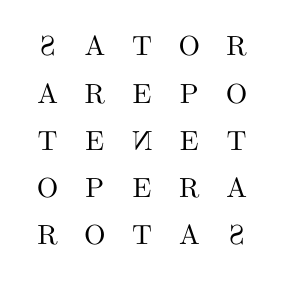
\begin{tikzpicture}[scale=0.6] % Adjust the scale factor as needed
    % Draw the Sator Square
    % \draw (0,0) grid (5,5);
    
    % Words in the Sator Square
    \node at (0.5,4.5) {\reflectbox{S}};
    \node at (1.5,4.5) {A};
    \node at (2.5,4.5) {T};
    \node at (3.5,4.5) {O};
    \node at (4.5,4.5) {R};
    
    \node at (0.5,3.5) {A};
    \node at (1.5,3.5) {R};
    \node at (2.5,3.5) {E};
    \node at (3.5,3.5) {P};
    \node at (4.5,3.5) {O};
    
    \node at (0.5,2.5) {T};
    \node at (1.5,2.5) {E};
    \node at (2.5,2.5) {\reflectbox{N}};
    \node at (3.5,2.5) {E};
    \node at (4.5,2.5) {T};
    
    \node at (0.5,1.5) {O};
    \node at (1.5,1.5) {P};
    \node at (2.5,1.5) {E};
    \node at (3.5,1.5) {R};
    \node at (4.5,1.5) {A};
    
    \node at (0.5,0.5) {R};
    \node at (1.5,0.5) {O};
    \node at (2.5,0.5) {T};
    \node at (3.5,0.5) {A};
    \node at (4.5,0.5) {\reflectbox{S}};
\end{tikzpicture}
\caption{Sator square}
    \label{tab:sator}
\end{table}

\textit{Thaumaturgy} is the art of ``wonder working.'' This can either be associated with Christian, saintly miracles or with other magical practices. In his \textit{Mathematicall Praeface to Elements of Geometrie of Euclid of Megara}, John Dee refers to thaumaturgy as the art of assembling mechanical objects of mathematical design. These machines were often attributed to magic by the uninitiated.\footnote{\citet{thaumaturgy}} Here we find an attractive metaphor: by the rational enciphering of a text or the mathematical assemblage of an object, onlookers may be astounded as if by the conjuring of magic. We can then refer to the æsthetic project of Trevor Bača's music as \textbf{Rational Thaumaturgy}\footnote{This term is borrowed from the novel \textit{Jonathan Strange \& Mr Norrell} by Susanna Clarke, a book which tells a fictionalized history of England and magical scholarship. While in the novel the term \emph{rational thaumaturgy} comes to represent the intellectual activities of non-practicing magicians (a class of individual often derided by the practicing magicians), no such negative connotation is intended here.}\marginpar{This terminology represents a slight rebranding of the title of Trevor Bača's dissertation: \emph{Magic Constructivism.}} in contrast to Francisco Guerrero's \textbf{Scientistic Romanticism}.\footnote{Scientistic romanticism refers to Guerrero's tendency to fetishize mathematics or scientific structures without having as deep an understanding of them as, say, Iannis Xenakis. In this way, Guerrero has a faith in the scientific aspects of the work giving meaning, truth, or beauty to his works. The stance is a modernist faith in progress in science as opposed to Bača's stance of encoded communication.} The artist's statement on Bača's website reads:

\begin{quote}
    \singlespacing
``I understand my music as emotive encoding. I write because I feel an emotional compulsion to write — to give form to fantastic or impossible colors and shapes as sound and as pleasure — and, yet, when I write, I am intensely aware of the fact that I am setting up and taking apart a code. I write for different combinations of instruments in chamber and orchestral settings and the written score is an important part of how I work. The act of score preparation is, for me, an emotional effort deeply concerned with the weight and energy and physical charge of raw and vibrant sounds, and, in equal measure, a type of work that is surpassingly symbolic, intimately bound up with the networks of potential meaning set up by marks on the page. I reject any dichotomy that pits the analytic against the emotional. Symbols can, and do, cut like knives. And I work for a music that is everywhere an emotional play of symbols, complete with all the almost unworkable contradictions such a play of symbols carries.

I don't understand either the societal or psychological parts of the composer role. And I would just as soon replace it with some other type of work carrying some other type of baggage. Sorcery, perhaps. A special appeal to concentration, with concern for a secret language of symbols, a secret way of reading the events and details of the natural world. I want music to be an intensely shared and public experience. And I want the intensity of that experience to result, at least in part, from an effort of decipherment, and translation, on all our parts.

My music comes back again and again to a constellation of images, and desire. The beauty of reflected and refracted light. The relationships between code and power and time. The assertion of power and importance in an everyday type of living. The delicacy of flowers and their parts. And networks of people and our relationships. I believe that there is something utterly human in rendering flashes of these ideas as symbols on the page, designed specifically for experience in some other, potentially unknown, place.''\footnote{\citet{bacawebsite}}
\end{quote}

By comparison, Ferneyhough describes his use of formalization in the following way:

\begin{quote}
    \singlespacing
    ``I think the use of any structure is [...] to enable one to have a framework within which one can meaningfully work at any given moment [...] it is a state of affairs at any given moment, and if you have worked the systems properly, then you have left yourself enough freedom to be able to react in a totally individual, and spontaneously significant fashion. Structures for me are not there to produce material; they're there to restrict the situation in which I have to compose.''\footnote{\citet[62]{toop}}
\end{quote}

From this perspective, formalization need not be used to \emph{justify} compositional decisions, rather it provides a situation which \emph{provokes} creative thinking. This is the aspect of modernist structuralism which I find the most exciting and the reason I specifically sought a loose but formalizeable approach to large-scale form.

\section{Rational Thaumaturgy}

While it certainly can be said that composers like Milton Babbitt, Francisco Guerrero, or Iannis Xenakis sought a scientistic justification for their artistic goals, the same cannot be said of composers such as Jean Barraqué, Pierre Boulez, Brian Ferneyhough, or Trevor Bača; whose use of systematic operations is disguised by a degree of composerly agency to modify the results of systematized products or through the implementation of ``cannibalizing'' systems which disguise themselves and cannot be reverse-engineered through analysis without recourse to sketch materials. The magical metaphor of \emph{Rational Thaumaturgy}, then, opens up an æsthetic category under the broader heading of modernism which encompasses works of this type which make use of modernist techniques and principles without the ethea of futurism or scientism which are often associated with such techniques.

\subsection{Analysis Beyond the Catalogue}

How should such a music be analyzed? What does an analysis intend to reveal? Analysis is an art-form in itself; sometimes revealing more about the orientations of the analyst than of anything substantive in the work itself. Should an analysis reveal the generative process of a work, consistencies within the behavior of a work or a group of works? What about the cultural context? All of these seem to be valuable avenues of exploration but perhaps analytic focus should be constrained to a specific category rather than aiming for unending comprehensiveness.

In the past I have struggled with understanding the nature and process of music analysis. What is music analysis and what is it for? In university we are often trained in a kind of rote analysis of labeling. However analysis is more than the mere identification of elements within a composition; the purpose of analysis is the understanding of musical style.\footnote{\citet[1]{white}} Pierre Boulez makes an interesting proposal for a different kind of analysis:

\begin{quote}
\singlespacing
``What is much more important in this case is the dialectic of composition [...] what may be called figured, or `ciphered,' analyses of this music are legion [...]. What is rewarding is to observe the dialectic of events, to obtain a bird's-eye view of the whole procedure and see how the composer contrives to formulate his thinking by means of such a system — that really does open up many more lines of inquiry.''\footnote{\citet[116]{boulez}}
\end{quote}

The nature of an analytic expression is primarily defined by the profession of the author. A musicologist might produce an analysis in order to say something about history or culture, a theorist might desire to communicate something about the mathematical properties latent in a musical schema, or a composer might wish to reveal properties of compositional craft which they find beautiful and therefore valuable. \marginpar{I think I have only been able to learn the craft of composition through the analysis of music and subsequent assimilation or rejection of the revealed properties of a work.} Boulez suggests that the indentification and labeling of materials and structures ought only to be done in service of understanding the transformation or interralatedness of structures across the whole of a composition:

\begin{quote}
\singlespacing
``Far the most important thing is to observe the existence of points shared 
 by different structures, and to mark the different areas of a work composed of such-and-such characteristics; to see how, in one section, certain features are avoided only to be concentrated in a future development; to follow, for instance, the interferences that may arise between forms or structures.''\footnote{\citet[117]{boulez}}
\end{quote}

\subsubsection{False Analysis}

The above references to Pierre Boulez's perspective on analysis ought to be problematized in view of his encouragement of ``false analysis.''

\begin{quote}
    \singlespacing
    ``The most seductive situation is to create a labyrinth from another labyrinth, to superimpose one's own labyrinth on the composer's: not to try in vain to reconstitute his method. A productive analysis is probably, in the most casual sense, a false analysis, which finds in the work not a general truth, but a particular, transitory truth, and [the analyst] grafts his own imagination on the imagination of the composer analysed.''\footnote{\citet[88]{boulez-language}}
\end{quote}

In his book \emph{The Musical Language of Pierre Boulez}, Jonathan Goldman gives the example of Stockhausen's analysis of Anton Webern's opus 28, wherein a spatial metaphor is taken up as a tool to analyze Webern's contrapuntally-produced densities, as an analysis which Boulez found both false and highly productive.\footnote{\citet[89]{boulez-language}} In the analytic chapters of this dissertation, I have not consciously engaged in deliberately false interpretations of the musical works in question. In the spirit of Boulez, I have developed an analytic framework which, when faced with musical structures which are not easily categorized by traditional means, aims for a deeper understanding of the works than a mere catalogue\marginpar{I am, however, a fan of catalogues. I once produced a several-thousand page document of all possible 12-tone equal-tempered sonorities of sizes 1-6 and every possible closed voicing of each sonority which I titled \emph{A Collection of Field Guides of Reasonably Calculable Pitch Objects,} a breathtaking document which revealed to me the fundamentally arbitrary nature of any musical choice, not only the choice of harmony and voicing. I admire the aura of botanical or avian field guides.} of pitch-class sets, rhythm series, or other identifiable, surface-level structures. Importantly, this framework has provided me with a way of imagining the development of form and material within my own compositional practice.

\subsubsection{Methodology}

In order to understand the formal characteristics of Barraqué's \textit{Sonate pour piano}, Guerrero's \textit{Rhea}, and Bača's \textit{Akasha}, I first needed to be able to identify the different thematic materials present throughout each work. I needed to prove the identity of these materials by analyzing their structures. Once the materials were taxonomized, it became possible to identify aspects of the large-scale form. In order to study the works at hand, I consulted scores, recordings, and sketch materials for each work and when no sketch material was available, I consulted other analysts' descriptions of sketches. I considered known techniques of each composer to suggest possible interpretations of the music. Both Francisco Guerrero Marín and Trevor Bača, developed compositional workflows in which they defined large-scale formal structures early and specified local musical events later. This meant that I was often able to consult the composer's outline of the work and use the score to prove the adherence (or lack of it) to the sketch. The composers assessed in this dissertation largely follow Iannis Xenakis' phases of a musical work:

\begin{enumerate}
  \item Initial conceptions
  \item Definition of the sonic entities: E\textsubscript{r}(c, h, g, u)\footnote{Where E\textsubscript{r} is a sonic entity at a point in multi-dimensional space provided by the vector elements (c, h, g, u), c=timbre or instrumental family, h=pitch, g=intensity of sound, and u=duration of sound}
  \item Definition of the transformations
  \item Microcomposition
  \item Sequential programming
  \item Implementation of calculations
  \item Final symbolic result
  \item Sonic realization\footnote{\citet[22]{xenakis}}
\end{enumerate}

Xenakis acknowledged the permutability of certain of these steps. While analyzing Brian Ferneyhough's \textit{Lemma-Icon-Epigram}, Richard Toop discusses his motivations for performing any kind of analysis on a work. Among these motivations, he mentions:

\begin{quote}
\singlespacing
``My own primary interest in analysis is as a means of reconstructing the creative process: of showing not just how a thing is done, but why. With composers like Boulez or Stockhausen it is often possible—though not really desirable—to do this without recourse to sketches; with Ferneyhough, for reasons that will become apparent, I believe this not to be the case.''\footnote{\citet[54]{toop}}
\end{quote}

The same is true for the composers discussed in this dissertation. I am also interested in reconstructing the creative process and to do so, in the cases of Guerrero and Bača, more than the score alone is required. %As seen later in this chapter, other kinds of analysis could be performed on these works; however, the kind of study I wanted involved understanding the formalized aspects of the compositions.

\subsubsection{Taxonomy}

Many alternative taxonomies can be used to classify things. Should animals be classified by their morphology or their genetics? The genetic analysis of the animal kingdom reveals many cases of both convergent and divergent evolution. Much can be learned about the history and potential future of our world through this kind of study. However, in many cases it may be more practical for the average individual to categorize things in a different way. The hippopotamus and the whale may be each other's closest common ancestor, but it is likely more functional for people outside of a scientific context to categorize them separately as water animals and land animals.\footnote{\citet{hippo}} In the same way, music analysis could take several routes. Is it more useful to categorize variations of themes based on the generative processes which bring them about, or should the perceived effect be the more important guiding principle? These questions should be considered on a case-by-case basis depending on the needs of a particular analysis. In the case of the analyses I performed in the preparation of this dissertation, I took the approach of searching for the genetic relationships between materials. %As a composer, I take a particular interest in the compositional processes performed by other composers. While a listening analysis of the works could be performed without access to archives of sketch materials, my own compositions came to be informed by the compositional techniques developed by Barraqué, Guerrero, and Bača.

\subsubsection{Analyzing Digital Sketch Material}

Ross Feller suggests that analyzing digital sketch material can be fraught due to the lack of preservation of the process of editing the file.\footnote{\citet[176]{sketches}} This is certainly the case of Francisco Guerrero's works which made use of computers, the material for which is likely lost, but in the case of Trevor Bača's works, a kind of compromise is at play. While every single keystroke — every deletion and revision — is not preserved, a version history is available. It is possible to see the project develop as it is saved after important periods of modification. Sometimes these stages are not worth observing as they simply represent the next day's worth of compositional effort. We can see passages reconfigured in endless iterations, to the point of becoming white noise: a flurry of action meaningless to the analyst.

\subsection{Form}

Before performing analysis, it is important for the analyst to establish criteria by which different compositions can be measured.

\subsubsection{Why Form?}

I am searching for a method which allows me to control both large-scale and local musical elements in a formalized manner, while activating the sense of form through interaction with memory. Much music which I hear as perceptually formless is still incredibly powerful. I think not only of Barraqué's \textit{Sonate}, but also of \textit{Occam Océan} by Éliane Radigue or \textit{Divisio Spiralis} by Catherine Lamb, whose glacially slow changes in harmony and totally static, un-activated rhythmic language produce a meditative deadening of the language-using part of my brain. Nevertheless, I find that the primary musical experience I crave involves the appearance of recurrent relationships between disparate moments within a piece—the sudden flash of a remembered motif like a bird in the understory of a dense forest.

\subsubsection{What is Form?}

The Harvard Dictionary of Music makes a distinction between the categories of ``form \textit{in} music'' and ``form(s) \textit{of} music.''\footnote{\citet[326-328]{dictionary}} \textbf{Form} refers to the fact that all art, including music, consists of elements arranged in an orderly fashion according to obvious or subtle principles, while \textbf{musical forms} refer to specific, culturally recurrent formal structures. Form, then, is the succession of events across the timeline of a work.\footnote{Possibly even a timeline of a single event.} I would like to add terms of relativity to the definition of form. \textit{Latent form} can refer to organizational features which a listener does not perceive in a given listening and \textit{activated form} can refer to structural elements which are discerned by the listener. These terms need not refer to some ontological ``knowability'' of musical features, as much music perception is dependant upon training and cultural exposure;\footnote{\cite[137]{psychology}} rather, the relativity of these terms comes to refer to specific individual experiences.

\subsubsection{Vers une Métaforme}

It can be useful to establish a vocabulary by which aspects of the compositional structure are referred.\footnote{To continue the magical metaphor, the magical system described in Ursula K. Le Guin's \textit{Earthsea} novels requires the knowledge of the true name of an object in order to manipulate it. Perhaps the same could be seen here: control of musical features is possible when they are known and deliberately deployed.} I attempt here to establish a framework for the analysis of music which is not from the tonal, motivic, or thematic practices of older Western classical music.\footnote{Certainly these concepts could be fruitfully applied to that music!} The smallest components of a piece of music are \textbf{points}. Points represent individual notes which have various sounding parameters of pitch, duration, intensity, timbre, and possibly qualities such as the method of sound production on a specific instrumental body. Points can be collected into \textbf{groups}. These groups may or may not behave exactly as described by Stockhausen, but a group can be seen as a collection of points which are perceived as a unified event in the memory stream. A group can be as small as a motif, the size of a figure, or as long as a phrase. Stockhausen considered the maximum size of a group to be eight notes;\footnote{\citet[40]{stockhausen}} however, given a closer relationship between points in a group, the statistical impression of much larger collections of points can be held in memory, although at a lower fidelity. Exactly at what point a group becomes a \textbf{mass} is largely contextual to the musical event and relative to the individual listener. While a composition must comprise at least one point which forms at least one group, compositions which feature greater variety within their landscape can be subdivided into more elements, whose behavior can be described in characteristic ways. %Certainly, a composition may or may not be comprised of these elements and an analysis of a work can make use of understanding the choice to deploy or not to deploy certain of these structures.

A sufficient level of consistency or relatedness between points in a group or mass—that is its having a high degree of salience—qualifies a group to be considered a \textbf{statement} of a \textbf{material}; a material being a diachronic, abstract set of criteria, possibly formalized as rules by which musical events can be grouped by their adherence to said criteria, and a statement being a particular, localized event which exhibits the characteristics of a given material. An \textbf{event group} refers to the collection of statements of a given material throughout the course of a piece. 

Statements of different materials must necessarily transition from one to the other. Some transition techniques summarized in the following figures include, but are not limited to \textit{Microformal}, \textit{Oppositional}, \textit{Evolutional}, \textit{Interruptive}, \textit{Tuilage}, \textit{Ligature}, and \textit{Incised/Imbricated} statements of materials. These types take on slightly different forms when dealing with more than two materials and in ensemble contexts, the boundaries between the stages of transition may be abrupt across the ensemble or staggered between instruments. We will see in the following chapters that Guerrero has a preference for oppositional transitions with staggered boundaries and Bača deploys numerous statement types, particularly tuilage transitions.

\begin{figure}[H]
    \centering
\begin{tikzpicture}
    \draw[pattern=crosshatch dots, pattern color=gray] (0,0) rectangle (6,1);
    \node (n1) at (0.5,1.25) {(AB)};
    \draw (1,1.25) -- (5.85,1.25);
\end{tikzpicture}
    \caption{Microformal: Many small instances of A and B}
    \label{fig:microformal}
\end{figure}

\begin{figure}[H]
    \centering
\begin{tikzpicture}
    \draw[pattern=north east lines, pattern color=blue] (0,0) rectangle (3,1);
    \node (n1) at (0.5,1.25) {A};
     \draw (1,1.25) -- (2.85,1.25);
    \draw[pattern=crosshatch, pattern color=orange] (3,0) rectangle (6,1);
    \node (n1) at (3.5,1.25) {B};
     \draw (4,1.25) -- (5.85,1.25);
\end{tikzpicture}
    \caption{Oppositional: A is abruptly contrasted by B}
    \label{fig:contrast}
\end{figure}

\begin{figure}[H]
    \centering
\begin{tikzpicture}
    \draw[pattern=north east lines, pattern color=blue] (0,0) rectangle (2,1);
    \node (n1) at (0.5,1.25) {A};
     \draw[->] (1,1.25) -- (1.85,1.25);
    \draw[pattern=crosshatch dots, pattern color=gray] (2,0) rectangle (4,1);
    \node (n1) at (2.5,1.25) {(Ab)};
     \draw[->] (3,1.25) -- (3.85,1.25);
    \draw[pattern=crosshatch, pattern color=orange] (4,0) rectangle (6,1);
    \node (n1) at (4.5,1.25) {B};
     \draw (5,1.25) -- (5.85,1.25);
\end{tikzpicture}
    \caption{Evolutional: A becomes B (or more like B)}
    \label{fig:evolution}
\end{figure}

\begin{figure}[H]
    \centering
\begin{tikzpicture}
    \draw[pattern=north east lines, pattern color=blue] (0,0) rectangle (3,1);
    \node (n1) at (0.5,1.25) {A};
     % \draw (1,1.25) -- (2.85,1.25);
     \draw (1,1.25) node[anchor=north]{} -- (2.85,1.5) node[anchor=north]{} -- (2.85,1.05) node[anchor=south]{} -- cycle;
    \draw[pattern=crosshatch, pattern color=orange] (3,0) rectangle (6,1);
    \node (n1) at (3.5,1.25) {B};
    \draw (4,1.25) -- (5.85,1.25);
\end{tikzpicture}
    \caption{Interruptive: A (or A's process) is curtailed by B (but can begin again)}
    \label{fig:interrupt}
\end{figure}

\begin{figure}[H]
    \centering
\begin{tikzpicture}
    \draw[pattern=north east lines, pattern color=blue] (0,0) rectangle (3,1);
    \node (n1) at (0.5,1.25) {A};
    \draw (1,1.25) -- (2.85,1.25);
    \draw[pattern=crosshatch, pattern color=orange] (1.75,0) rectangle (4.75,-1);
    \node (n1) at (2.25,-1.25) {B};
    \draw (2.75,-1.25) -- (4.7,-1.25);
\end{tikzpicture}
    \caption{Tuilage: A is happening simultaneously with B}
    \label{fig:variegated}
\end{figure}

\begin{figure}[H]
    \centering
\begin{tikzpicture}
    \draw[pattern=north east lines, pattern color=blue] (0,0) rectangle (2,1);
    \node (n1) at (0.5,1.25) {A};
     \draw (1,1.25) -- (1.85,1.25);
    \draw[pattern=north east lines, pattern color=blue] (2,0) rectangle (4,1);
    \draw[pattern=north west lines, pattern color=orange] (2,0) rectangle (4,1);
    \node (n1) at (2.5,1.25) {\{AB\}};
     \draw (3,1.25) -- (3.85,1.25);
    \draw[pattern=crosshatch, pattern color=orange] (4,0) rectangle (6,1);
    \node (n1) at (4.5,1.25) {B};
     \draw (5,1.25) -- (5.85,1.25);
\end{tikzpicture}
    \caption{Ligature: characteristics of A and B are recombined to form a new compound material}
    \label{fig:ligature}
\end{figure}

\begin{figure}[H]
    \centering
\begin{tikzpicture}
    \draw[pattern=north east lines, pattern color=blue] (0,0) rectangle (2,1);
    \node (n1) at (0.5,1.25) {A};
     \draw (1,1.25) -- (1.85,1.25);
    \draw[pattern=crosshatch, pattern color=orange] (2,0) rectangle (3,1);
    \node (n1) at (2.5,1.25) {b};
     % \draw (3,1.25) -- (3.85,1.25);
     \draw[pattern=north east lines, pattern color=blue] (3,0) rectangle (4,1);
    \node (n1) at (3.5,1.25) {a};
     % \draw (3,1.25) -- (3.85,1.25);
    \draw[pattern=crosshatch, pattern color=orange] (4,0) rectangle (6,1);
    \node (n1) at (4.5,1.25) {B};
     \draw (5,1.25) -- (5.85,1.25);
\end{tikzpicture}
    \caption{Incised/Imbricated: A is cut into / layered between B}
    \label{fig:incision}
\end{figure}

%While a composition could be monothematic, or containing only one definite material, the works under consideration in this dissertation contain many.
Over the course of a work, we can consider various formal ``moves'' under the labels \textbf{Repetition}, \textbf{Recurrence}, \textbf{Variation}, and \textbf{Contrast}.\footnote{Note that the \textit{contrast} formal move could produce genuinely novel material or may operate in conjunction with recurrence and variation of previously exposited material.} Repetition is the literal enclosure of a passage of music within repeat barlines to be repeated one or more times in immediate succession; recurrence is the non-contiguous, exact quotation of a passage of music; variation is the statement of a previously-heard material with some kind of alteration (perhaps part of a long-term linear trajectory); and contrast is the succession of one material by a different material. Variation can encompass what is traditionally called motivic development, but can also encompass ``animation'' techniques.

A statement can be considered as having \textbf{animation} when it occurs with some actively changing parameter like pitch up or down, dynamics loud or soft, rhythmic acceleration or deceleration, additive growth of durations, increase or decrease of texture density, expansion or contraction of figures in duration or pitch space, and decrease or increase of figuration such as incrementing the number of grace notes attached to sequential rhythmic events. All of these animations have the quality of reversibility.\footnote{Which is not necessarily the case for motivic development.} Non-motivic \textbf{development} is animation with a clear, statistically unidirectional teleology. Development can occur \textbf{locally}, within a particular statement of a material, or \textbf{long-term}: a narrative arc which is revealed across multiple appearances of a material. An example of a local development could be a 7-measure statement which gradually ascends in register. A long-term development could be a material which is gradually encrusted with a greater density of grace notes upon each of its statements.

Formalized music has a history of numeromancy, that is a modeling of sound-parametric space through the manipulation of numeric values. Certain operations on collections of values produce either a sense of stasis or a sense of motion. \textit{Permutative} operations which shuffle the order of elements in a sequence seem to produce stasis, while directionality seems to be produced by (not always linearly!) incrementing values. So the \textit{developmental} value of an operation depends on whether said operation has a tendency for perceptual stasis or directional energy.

Different materials can be assessed by the number of times they are repeated, and passages can be categorized by the density, or rate of change, within or between materials. A material which occurs more frequently in a work could potentially leave a greater impression in the mind of the listener than a material which occurs infrequently, however this could be counteracted by a severe slowing of the rate of change. A material which only occurs once in a piece but takes up half of the total time of the performance stands a chance of leaving the greatest impression upon the audience.

In my personal, compositional criteria, it is integral to avoid a perception of sameness. I have found that it is important to use an irregular distribution of the aforementioned techniques at varying densities and rates of change. Asymmetry and irregularity are key elements to my impression of the success of the memory experience of a formal structure.

\subsection{Analysis towards Creation}

In the analyses in the following chapters, I hope to show some of the techniques used by Jean Barraqué, Francisco Guerrero and Trevor Bača to formalize the relationships between statements within event groups, and how clear distinctions between materials are used to define sections of a work,\footnote{Works like \textit{Rhea} and \textit{Akasha}, through their constant use of simultaneous material polyphony represent variegated form while Barraqué's \textit{Sonate} is more accurately described as exhibiting sectional form.} after which I will describe two examples from my compositional practice which take explicit inspiration from the structures discovered in these works.